\documentclass{article}

\usepackage[final]{neurips_2020}

\usepackage[utf8]{inputenc}
\usepackage[T1]{fontenc}
\usepackage{hyperref}
\usepackage{url}
\usepackage{booktabs}
\usepackage{amsfonts}
\usepackage{amsmath}
\usepackage{nicefrac}
\usepackage{microtype}
\usepackage{graphicx}
\usepackage{xcolor}
\usepackage{multirow}
\usepackage{kotex}   % 한국어 렌더링 (XeLaTeX 필요)

\usepackage{tikz}
\usetikzlibrary{arrows.meta}

\title{
  Difficulty-Aware Language Routing and \\
  Cross-Lingual Self-Consistency \\
  for Korean Mathematical Reasoning \\
  \vspace{1em}
  \small{\normalfont Korea University COSE461 Final Project}
}

\author{%
  \small
  \begin{tabular}{ccc}
    \textbf{Lee Yunje} & \textbf{Kim Sangjun} & \textbf{Won Junseo} \\[3pt]
    {\footnotesize\mdseries Department of Data Science} &
    {\footnotesize\mdseries Department of Data Science} &
    {\footnotesize\mdseries Department of Data Science} \\[1pt]
    {\footnotesize\mdseries Team 20} &
    {\footnotesize\mdseries Team 20} &
    {\footnotesize\mdseries Team 20} \\[1pt]
    {\footnotesize\mdseries 2022320317} &
    {\footnotesize\mdseries 2022320306} &
    {\footnotesize\mdseries 2022320302}
  \end{tabular}%
}


\begin{document}

\maketitle

\begin{abstract}
Small language models reason markedly better in English than in Korean
on mathematical word problems. We trace part of this gap to the
distillation pipeline itself: even a strong teacher (Gemini) produces
lower-quality chain-of-thought (CoT) in Korean (85.7\% correct) than in
English (97.5\%), so naively distilling Korean CoT transfers a noisier
signal. We address this with a two-stage cross-lingual framework. At
the \textbf{data level}, our main contribution \textbf{Difficulty-Aware
Language Routing (DALR)} decides, per problem, whether to learn from a
Korean or an English teacher CoT based on teacher correctness: English
CoT is used only as a ``bridge'' on problems the Korean teacher fails.
A controlled ablation (DALR vs.\ random English placement) shows DALR's
gain stems from \emph{where} English reasoning is routed, not from
added data. At the \textbf{inference level}, we apply
\textbf{Cross-Lingual Self-Consistency (XLSC)}, sampling each problem
in both Korean and English from the same DALR-trained model and
aggregating by majority vote. On HRM8K (Korean) with Qwen2.5-3B,
DALR achieves the best single-model Korean accuracy (61.79\%), and
DALR + XLSC reaches 69.90\% (+16.00 pts over base); the XLSC
inference-time gain reproduces on Llama-3.2-3B (+8.19) and
EXAONE-3.5-2.4B (+8.79).
\end{abstract}


\section{Introduction}
Large language models demonstrate strong multi-step mathematical
reasoning, but small models (e.g.\ 3B parameters) lag far behind, and
the gap is worse outside English~\citep{shi2023mgsm}. For
Qwen2.5-3B-Instruct, the model solves \textbf{71.65\%} of English
problems (GSM8K~\citep{cobbe2021gsm8k}) but only \textbf{53.90\%} of
Korean problems (HRM8K~\citep{ko2025hrm8k}). Practical deployments
often cannot afford large models yet must serve non-English users, so
this gap is consequential.

A standard remedy is knowledge distillation: a strong teacher
generates chain-of-thought (CoT) solutions~\citep{wei2022cot}, and a
small student is fine-tuned on them. However, in the cross-lingual
setting, the teacher itself is weaker in Korean: on our training set,
Gemini produces correct CoT for 97.5\% of English problems but only
85.7\% of Korean problems. Distilling Korean CoT therefore transfers
a noisier signal than English, leaving substantial room for
improvement in Korean. Existing cross-lingual remedies act mostly at
inference time, such as English-pivot translation or cross-lingual
prompting~\citep{qin2023crosslingual,chai2025xcot}, and leave the
student's underlying weights monolingual; we instead intervene at the
training-data construction stage so that the cross-lingual signal is
internalized.

This motivates our central question: \emph{can the teacher's---and a
model's---stronger English reasoning be used to improve a small
student's Korean mathematical reasoning?} Our working assumption is
that mathematical \emph{logic} is largely language-agnostic, so
connecting English reasoning patterns to Korean problems should help.

We pursue this through a two-stage cross-lingual framework. At the
\textbf{data level}, our main contribution \textbf{DALR} routes each
problem to a Korean or English teacher CoT based on teacher
correctness. At the \textbf{inference level}, \textbf{XLSC} samples
from the same DALR-trained model in both languages and aggregates by
majority vote.

\paragraph{Contributions.}
\begin{itemize}
  \item We propose \textbf{DALR}, a difficulty-aware data-construction
  method for cross-lingual CoT distillation, and show via a controlled
  ablation that its gains come from \emph{routing}, not added data.
  \item We propose \textbf{XLSC}, an inference-time aggregation method
  that exploits the bilingual reasoning capability instilled by DALR.
  \item Empirically, DALR raises HRM8K accuracy from \textbf{53.90\%}
  to \textbf{61.79\%} on Qwen2.5-3B, and DALR + XLSC reaches
  \textbf{69.90\%} (+16.00 pts over base); the XLSC inference-time
  gain reproduces on Llama-3.2-3B (+8.19) and EXAONE-3.5-2.4B (+8.79).
\end{itemize}

\section{Related Work}
\paragraph{Chain-of-thought and its distillation.}
Chain-of-thought (CoT) prompting elicits intermediate reasoning steps
in large language models and substantially improves multi-step
mathematical accuracy~\citep{wei2022cot}. A subsequent line of work
\emph{distills} this ability into smaller students by fine-tuning
them on teacher-generated CoT
\citep{magister2023teaching, ho2023large, hsieh2023distilling}.
Our pipeline is an instance of CoT distillation, but unlike prior
work that fixes a single teacher language for the whole training set,
DALR chooses the CoT language \emph{per problem} based on teacher
correctness.

\paragraph{Cross-lingual reasoning.}
Reasoning transfers unevenly across languages: even strong models
solve math problems markedly better in English than in lower-resource
languages~\citep{shi2023mgsm}. Existing remedies typically act at
\emph{inference} time, by translating non-English questions to
English before reasoning (English-pivot) or by cross-lingual prompting
\citep{qin2023crosslingual, chai2025xcot, huang2023languages}, or at
the \emph{instruction-tuning} level with multilingual CoT data
\citep{chen2024breaking}. DALR instead acts at the
\emph{training-data construction} level: cross-lingual signal is
selected per problem and internalized in the student weights, rather
than appended at inference.

\paragraph{Self-consistency.}
Self-consistency samples multiple chains from one model and selects
the majority answer~\citep{wang2022selfconsistency}, trading compute
for accuracy. XLSC extends this idea \emph{cross-lingually}: instead
of $N$ chains in a single language, it samples in both Korean and
English from the same DALR-trained model and votes over the union,
exploiting errors that decorrelate across
languages~\citep{huang2023languages}.

\paragraph{Data selection for distillation.}
A complementary line filters teacher CoT by correctness, keeping only
chains whose final answer matches the gold
label~\citep{zelikman2022star}. DALR builds on this rejection-sampling
view but treats teacher \emph{language} as an additional axis of
selection: when the Korean teacher fails, the English CoT is
substituted as a ``bridge,'' so teacher failure itself serves as a
per-problem difficulty signal.


\section{Approach}
\subsection{Overview}
We train a single small student with DALR-constructed data and
aggregate its predictions at inference with XLSC. The two stages
inject cross-lingual signal at different points: DALR at training
time, deciding the CoT language per problem based on teacher
correctness, and XLSC at inference time, sampling chains in both
Korean and English from the same model and majority-voting.
Figure~\ref{fig:pipeline} illustrates the framework end-to-end. The
data routing in Stage~1 (Section~\ref{sec:dalr}) is our main
methodological contribution; the inference-time aggregation in
Stage~2 (Section~\ref{sec:xlsc}) is a natural complement that
exploits the bilingual capability instilled by Stage~1.

\begin{figure}[t]
\centering
\resizebox{\textwidth}{!}{%
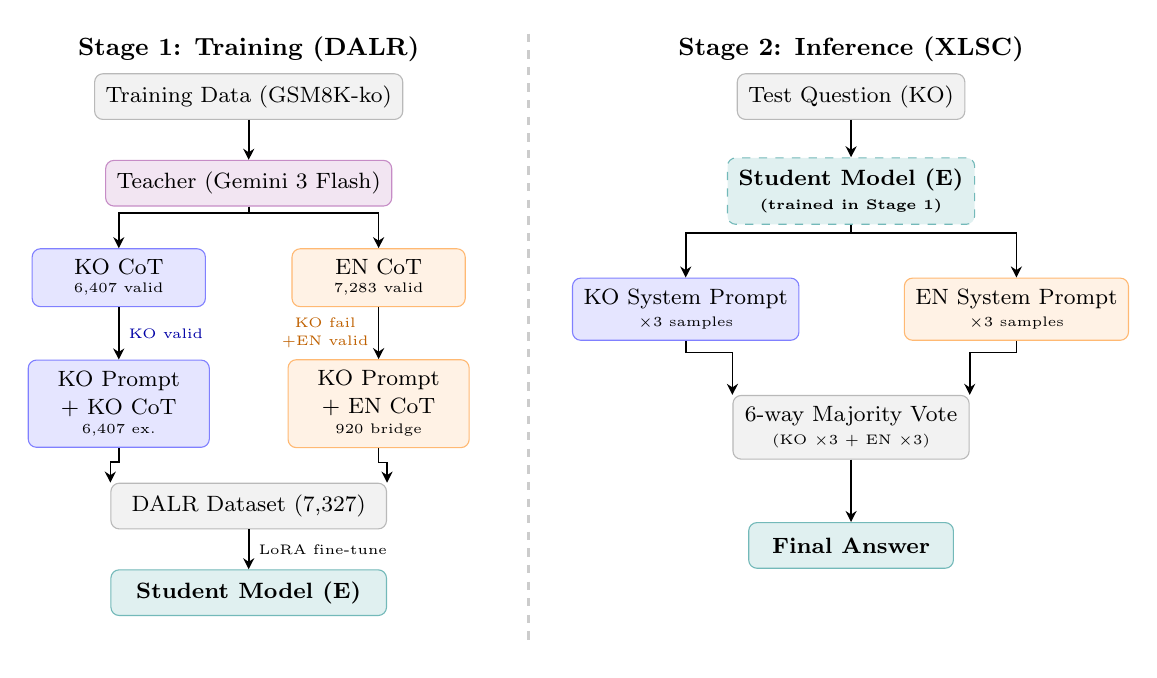
\begin{tikzpicture}[
  font=\footnotesize,
  box/.style={rectangle, rounded corners=3pt, draw=black!50, fill=white,
              text centered, inner sep=4pt,
              minimum width=2.4cm, minimum height=0.58cm},
  kobox/.style={box, fill=blue!10, draw=blue!50},
  enbox/.style={box, fill=orange!10, draw=orange!55},
  gbox/.style={box,  fill=gray!10, draw=gray!55},
  sbox/.style={box,  fill=teal!12, draw=teal!55, font=\footnotesize\bfseries},
  tbox/.style={box,  fill=violet!10, draw=violet!45},
  arr/.style={-{Stealth[length=4pt,width=4pt]}, semithick},
]

%% ---- Stage 1 label ----
\node[font=\small\bfseries] at (3.15, 0.6) {Stage 1: Training (DALR)};

%% ---- Stage 1 nodes ----
\node[gbox, minimum width=3.5cm] (train)   at (3.15,  0.0)
  {Training Data (GSM8K-ko)};
\node[tbox, minimum width=3.5cm] (teacher) at (3.15, -1.1)
  {Teacher (Gemini 3 Flash)};
\node[kobox, minimum width=2.2cm] (kocot)  at (1.5, -2.3)
  {\shortstack{KO CoT\\\tiny 6,407 valid}};
\node[enbox, minimum width=2.2cm] (encot)  at (4.8, -2.3)
  {\shortstack{EN CoT\\\tiny 7,283 valid}};
\node[kobox, minimum width=2.3cm] (kopath) at (1.5, -3.9)
  {\shortstack{KO Prompt\\+ KO CoT\\\tiny 6,407 ex.}};
\node[enbox, minimum width=2.3cm] (enpath) at (4.8, -3.9)
  {\shortstack{KO Prompt\\+ EN CoT\\\tiny 920 bridge}};
\node[gbox,  minimum width=3.5cm] (dalr)   at (3.15, -5.2)
  {DALR Dataset (7,327)};
\node[sbox,  minimum width=3.5cm] (student) at (3.15, -6.3)
  {Student Model (E)};

%% ---- Stage 1 arrows ----
\draw[arr] (train) -- (teacher);
\draw[arr] (teacher.south) -- ++(0,-.08) -| (kocot.north);
\draw[arr] (teacher.south) -- ++(0,-.08) -| (encot.north);
\draw[arr] (kocot) -- node[right, font=\tiny, blue!65!black]{KO valid} (kopath);
\draw[arr] (encot) -- node[left,  font=\tiny, orange!75!black, align=center]
           {\shortstack{KO fail\\+EN valid}} (enpath);
\draw[arr] (kopath.south) -- ++(0,-.18) -| (dalr.north west);
\draw[arr] (enpath.south) -- ++(0,-.18) -| (dalr.north east);
\draw[arr] (dalr) -- node[right, font=\tiny]{LoRA fine-tune} (student);

%% ---- Divider ----
\draw[very thick, dashed, gray!40] (6.7, 0.8) -- (6.7, -7.0);

%% ---- Stage 2 label ----
\node[font=\small\bfseries] at (10.8, 0.6)
  {Stage 2: Inference (XLSC)};

%% ---- Stage 2 nodes ----
\node[gbox,  minimum width=2.8cm] (testq)  at (10.8,  0.0)
  {Test Question (KO)};
\node[sbox,  minimum width=3.0cm, dashed]  (stud2)  at (10.8, -1.2)
  {\shortstack{Student Model (E)\\\tiny (trained in Stage 1)}};
\node[kobox, minimum width=2.6cm] (kosamp) at (8.7, -2.7)
  {\shortstack{KO System Prompt\\\tiny $\times 3$ samples}};
\node[enbox, minimum width=2.6cm] (ensamp) at (12.9, -2.7)
  {\shortstack{EN System Prompt\\\tiny $\times 3$ samples}};
\node[gbox,  minimum width=3.0cm] (vote)   at (10.8, -4.2)
  {\shortstack{6-way Majority Vote\\\tiny (KO $\times 3$ + EN $\times 3$)}};
\node[sbox,  minimum width=2.6cm] (ans)    at (10.8, -5.7)
  {Final Answer};

%% ---- Stage 2 arrows ----
\draw[arr] (testq) -- (stud2);
\draw[arr] (stud2.south) -- ++(0,-.10) -| (kosamp.north);
\draw[arr] (stud2.south) -- ++(0,-.10) -| (ensamp.north);
\draw[arr] (kosamp.south) -- ++(0,-.15) -| (vote.north west);
\draw[arr] (ensamp.south) -- ++(0,-.15) -| (vote.north east);
\draw[arr] (vote) -- (ans);

\end{tikzpicture}%
}
\caption{Two-stage cross-lingual framework.
\textbf{Stage~1 (DALR):} each training problem is routed to a Korean
teacher CoT if valid, or an English ``bridge'' CoT otherwise; the
920 bridge examples target problems the Korean teacher fails.
\textbf{Stage~2 (XLSC):} at inference, the same student generates
three Korean and three English chains per problem and aggregates by
majority vote over the resulting six answers.}
\label{fig:pipeline}
\end{figure}


\subsection{Difficulty-Aware Language Routing (DALR)}
\label{sec:dalr}

The cross-lingual setting introduces a structural mismatch in CoT
distillation: the teacher is unevenly competent across languages.
On our Korean training set, Gemini produces a correct chain for only
85.7\% of problems in Korean versus 97.5\% in English, a 12-point
gap. Distilling Korean CoT as-is therefore propagates a noisier
signal to the student on the problems where the teacher itself
struggles, presumably also where the student struggles---consistent with
the per-difficulty analysis in Section~\ref{sec:analysis}. DALR turns this gap into
a \emph{free per-problem difficulty signal}: when the teacher fails
in Korean, the problem is hard for Korean reasoning, so we
substitute the English CoT as a higher-quality target rather than
discarding the problem or fine-tuning on an unreliable Korean chain.

\paragraph{Routing rule.}
For each Korean training problem $i$ we have the original Korean
question $q_i$, a Korean teacher CoT $c_i^{\text{KO}}$, an English
teacher CoT $c_i^{\text{EN}}$, and binary correctness flags
$v_i^{\text{KO}}, v_i^{\text{EN}} \in \{0,1\}$ from exact-match on
the final numeric answer. DALR emits exactly one training example
$t_i$ per problem:
\begin{equation}
\label{eq:dalr}
t_i \;=\;
\begin{cases}
(q_i,\ c_i^{\text{KO}},\ s^{\text{KO}}) & \text{if } v_i^{\text{KO}} = 1, \\[2pt]
(q_i,\ c_i^{\text{EN}},\ s^{\text{EN}}) & \text{if } v_i^{\text{KO}} = 0 \text{ and } v_i^{\text{EN}} = 1, \\[2pt]
\varnothing\ (\text{discarded})         & \text{otherwise},
\end{cases}
\end{equation}
where $s^{\text{KO}}$ and $s^{\text{EN}}$ are the Korean and English
system prompts respectively. The user question $q_i$ is always
Korean; only the CoT language and the system prompt change. The
student is fine-tuned with the system prompt matching the target
CoT language, so it learns to switch reasoning languages conditional
on prompt rather than on question language---a property we exploit
later for XLSC (Section~\ref{sec:xlsc}).
Figure~\ref{fig:dalr-example} illustrates both routing cases on
concrete GSM8K problems.

\begin{figure}[t]
\centering
\resizebox{\textwidth}{!}{%
\begin{tikzpicture}[
  font=\small,
  arr/.style={-{Stealth[length=4pt,width=3pt]}, semithick},
  darr/.style={-{Stealth[length=4pt,width=3pt]}, semithick, dashed, red!55},
  qbox/.style={rectangle, rounded corners=4pt, draw=gray!55, fill=gray!7,
               text width=4.8cm, inner sep=5pt, align=left},
  kocotbox/.style={rectangle, rounded corners=4pt, draw=blue!50, fill=blue!7,
                   text width=2.6cm, inner sep=5pt, align=left},
  encotbox/.style={rectangle, rounded corners=4pt, draw=orange!55, fill=orange!7,
                   text width=2.6cm, inner sep=5pt, align=left},
  trainbox/.style={rectangle, rounded corners=4pt, draw=teal!55, fill=teal!7,
                   text width=4.8cm, inner sep=5pt, align=left},
]

%% ===== Case 1: KO valid =====
\node[font=\small\bfseries] at (2.6, 0.55) {Case 1: KO CoT valid};

\node[qbox] (q1) at (2.6, -0.45) {
  {\scriptsize\textbf{Q (KO):} 리자는 버터 10\,kg 구매.
  초콜릿칩 $\tfrac{1}{2}$, 땅콩버터 $\tfrac{1}{5}$,
  남은 것의 $\tfrac{1}{3}$ 설탕 쿠키 사용. \textbf{남은 버터?}}
};

\node[kocotbox] (ko1) at (0.8, -2.7) {
  {\scriptsize\textbf{\textcolor{blue!70!black}{KO CoT}}~%
  \textcolor{green!50!black}{\bfseries\checkmark}}\\[3pt]
  {\tiny
  초콜릿칩: $10\times\tfrac{1}{2}=5$\\[1pt]
  땅콩버터: $10\times\tfrac{1}{5}=2$\\[1pt]
  사용 $5{+}2{=}7$, 남은 $3$\\[1pt]
  설탕: $3\times\tfrac{1}{3}=1$\\[1pt]
  $\mathbf{3{-}1=2}$\,kg}
};

\node[encotbox] (en1) at (4.4, -2.7) {
  {\scriptsize\textbf{\textcolor{orange!70!black}{EN CoT}}~%
  \textcolor{gray!55}{\scriptsize unused}}\\[3pt]
  {\tiny
  Choc: $10\times\tfrac{1}{2}=5$\\[1pt]
  PB: $10\times\tfrac{1}{5}=2$\\[1pt]
  Used 7, left $10{-}7{=}3$\\[1pt]
  Sugar: $3\times\tfrac{1}{3}=1$\\[1pt]
  $\mathbf{3{-}1=2}$\,kg}
};

\node[trainbox] (t1) at (2.6, -5.1) {
  {\scriptsize\textbf{Training:}}\\[3pt]
  {\tiny\texttt{[KO System Prompt]}\\[1pt]
  \textbf{Q:} 리자는 버터 10\,kg\,\ldots\\
  \textbf{A:} $\ldots$~$3{-}1{=}2$. 정답: \textbf{2\,kg}}
};

\draw[arr] (q1.south) -- ++(0,-.10) -| (ko1.north);
\draw[arr] (q1.south) -- ++(0,-.10) -| (en1.north);
\draw[arr] (ko1.south) -- ++(0,-.22) -| (t1.north west);

%% ===== Divider =====
\draw[thick, dashed, gray!35] (6.55, 0.85) -- (6.55, -6.1);

%% ===== Case 2: KO invalid (bridge) =====
\node[font=\small\bfseries, align=center] at (10.5, 0.55)
  {Case 2: KO CoT invalid~(bridge)};

\node[qbox] (q2) at (10.5, -0.45) {
  {\scriptsize\textbf{Q (KO):} 스나이더 씨 월수입의 40\%가
  집세. 월급 \$600 인상 후 집세 25\%로 감소.
  \textbf{이전 월수입은?}}
};

\node[kocotbox] (ko2) at (8.5, -2.7) {
  {\scriptsize\textbf{\textcolor{blue!70!black}{KO CoT}}~%
  \textcolor{red!60}{\bfseries$\times$}}\\[3pt]
  {\tiny
  비율 차: $40\%{-}25\%{=}15\%$\\[1pt]
  15\%가 \$600에 해당\\[1pt]
  $600\div0.15$\\[1pt]
  $=\mathbf{\$4{,}000}$~\textcolor{red!60}{(오답)}}
};

\node[encotbox] (en2) at (12.5, -2.7) {
  {\scriptsize\textbf{\textcolor{orange!70!black}{EN CoT}}~%
  \textcolor{green!50!black}{\bfseries\checkmark}}\\[3pt]
  {\tiny
  Let $p=$ prev.\ income\\[1pt]
  Rent fixed: $0.40p$\\[1pt]
  $0.40p{=}0.25(p{+}600)$\\[1pt]
  $0.15p{=}150$\\[1pt]
  $p=\mathbf{\$1{,}000}$}
};

\node[trainbox] (t2) at (10.5, -5.1) {
  {\scriptsize\textbf{Training (bridge):}}\\[3pt]
  {\tiny\texttt{[EN System Prompt]}\\[1pt]
  \textbf{Q:} 스나이더 씨 월수입의 40\%\,\ldots\\
  \textbf{A:} $0.40p{=}0.25(p{+}600)$,~$p{=}\mathbf{\$1{,}000}$}
};

\draw[arr] (q2.south) -- ++(0,-.10) -| (ko2.north);
\draw[arr] (q2.south) -- ++(0,-.10) -| (en2.north);

\draw[darr] (ko2.south) -- ++(0,-.30)
  node[right, font=\tiny, text=red!55!black]{discarded};

\draw[arr] (en2.south) -- ++(0,-.30) -| (t2.north);

\end{tikzpicture}%
}
\caption{Concrete illustration of DALR routing (Eq.~\ref{eq:dalr})
on two GSM8K training problems.
\textbf{Case~1} (Liza's butter): the Korean teacher CoT correctly
decomposes three fraction operations and reaches 2\,kg, becoming the
direct training target.
\textbf{Case~2} (Mrs.\ Snyder's income): the Korean CoT conflates
the 15-point percentage drop with the \$600 salary increase
(\$4,000 $\neq$ \$1,000); the English CoT sets up the correct
equation $0.40p = 0.25(p{+}600)$ and is substituted as a bridge.
The Korean question is unchanged in both cases.}
\label{fig:dalr-example}
\end{figure}

\paragraph{Dataset.}
Applied to GSM8K-ko's 7,473 training problems, Eq.~\ref{eq:dalr}
yields 6,407 Korean-CoT examples ($v^{\text{KO}}{=}1$), 920
English-bridge examples ($v^{\text{KO}}{=}0,\ v^{\text{EN}}{=}1$),
and 146 discarded problems where the teacher failed in both
languages (7,327 retained in total). The bridge rate (920/7,473 =
12.3\%) closely tracks the 14.3\% Korean teacher failure rate; the
residual 2.0\% gap is accounted for by these discards. We denote the resulting
fine-tuned model \textbf{E}; all baselines
(Section~\ref{sec:baselines}) share the student backbone, LoRA
configuration, and training hyperparameters, differing only in
dataset composition.

\paragraph{Design choices.}
Three design decisions distinguish DALR from related distillation
recipes. \emph{(i) Per-problem one-hot routing.} A bilingual mix
(Setup D) pools Korean and English chains in a 50:50 ratio without
regard to per-problem difficulty, so the choice of reasoning
language is undirected. DALR instead makes a per-problem decision
and emits exactly one target, the higher-quality language, for each
question; it is strictly smaller than D (7,327 vs.\ 12,814), yet
outperforms it (Section~\ref{sec:results}). \emph{(ii) Teacher
correctness as the difficulty signal.} Correctness is label-free,
requires no extra annotation, and generalizes to any teacher--student
pair. It also has a direct interpretation: if the strongest
available model cannot produce a verifiable Korean solution, the
Korean CoT for that problem is almost certainly low-quality
reasoning, while the English CoT \emph{is} verified.
\emph{(iii) Discard rather than fall back to a wrong chain.}
For the 146 problems where both teacher languages fail, DALR removes
the example outright instead of training on a known-wrong chain, a
small (2\%) cost in coverage in exchange for cleaner gradients.

\subsection{Cross-Lingual Self-Consistency (XLSC)}
\label{sec:xlsc}
DALR produces a model that reasons reliably in either Korean or
English, but a single greedy decode commits to one chain in one
language and inherits its errors. XLSC removes this commitment by
sampling in both languages from the \emph{same} DALR-trained model
and aggregating across them, exploiting the fact that Korean and
English chains traverse different intermediate steps for the same
problem and produce partially decorrelated errors
(Section~\ref{sec:analysis} quantifies this).

\paragraph{Aggregation rule.}
For each Korean test problem $q$, we draw $N$ chains under each
system prompt $s^L$, $L \in \{\mathrm{KO}, \mathrm{EN}\}$, from the
same DALR-trained model $\mathcal{M}_E$ at sampling temperature $T$,
and return the plurality answer over the resulting $2N$ extracted
numbers:
\begin{equation}
  c^L_k \sim \mathcal{M}_E(\cdot \mid s^L, q;\, T),
  \qquad
  \hat{y}_{\mathrm{XLSC}}(q) \;=\;
  \mathrm{mode}\!\left(
    \{\,\mathrm{extract}(c^L_k)\,\}_{\,L \in \{\mathrm{KO}, \mathrm{EN}\},\; k = 1,\dots,N}
  \right),
\end{equation}
where $\mathrm{extract}(\cdot)$ recovers the final numeric answer
from a chain and $\mathrm{mode}(\cdot)$ returns the most frequent
element (plurality vote) over the $2N$-element multiset.

\paragraph{Bilingual extraction.}
Because samples come in two languages but vote jointly, the answer
extractor must succeed on both: we apply two regular expressions in
parallel, one matching the Korean answer-marker phrase and one
matching its English equivalent (\texttt{answer is X}), with a
fallback to the last number in the chain. Without this bilingual
matching, chains ending in the other language's answer line would be
silently dropped from the vote.

\paragraph{Design choices.}
We use a single $\mathcal{M}_E$ rather than two monolingual
models---DALR already internalizes both languages---and weight all
$2N$ votes equally to avoid reintroducing the per-language reliability
gap that DALR was designed to neutralize. XLSC costs $2N$ forward
passes per problem versus $1$ for greedy decoding, purely at
inference.

\section{Experiments}

\subsection{Baselines}
\label{sec:baselines}
We design baselines to isolate one factor at a time.
\textbf{A (Base)} is unmodified Qwen2.5-3B-Instruct, the no-training
floor. \textbf{B (English-only)} and \textbf{C (Korean-only)}
fine-tune on the 7,283 English or 6,407 Korean teacher chains
respectively, the two ``obvious'' monolingual choices.
\textbf{D (Bilingual 50/50)} balances B and C 1:1 by sub-sampling
English down to the Korean count (12,814 examples, 6,407 of each),
exposing the student to both languages in equal proportion; D
answers whether undirected bilingual data alone suffices.
\textbf{E\_random} is a tightly matched control for DALR: identical
training pipeline, identical 920 English chains, but the English
chains are injected on \emph{randomly chosen Korean-solved}
problems---i.e.\ on problems where the Korean teacher already
succeeded, the opposite of DALR's routing principle---while
preserving the total of 7,327 examples. If DALR's gain were data
scaling, E and E\_random would tie; if it is routing, E should
dominate. All conditions share the student backbone, LoRA
configuration ($r=32$, $\alpha=64$), and training hyperparameters,
differing only in dataset composition.

\subsection{Data}
\paragraph{Training.}
GSM8K~\citep{cobbe2021gsm8k} provides 7,473 training and 1,319 test
problems in English grade-school mathematics. We use GSM8K-ko, a
machine-translated Korean version of the training split. The teacher
model (Gemini 3 Flash) generates chain-of-thought solutions
independently in English and Korean; we retain only solutions whose
final numeric answer matches the gold label (English: 7,283 valid
out of 7,473; Korean: 6,407 valid). Invalid Korean CoTs are replaced
by the corresponding English CoT in the DALR setup, or discarded
otherwise.

\paragraph{Evaluation.}
We evaluate on \textbf{HRM8K}~\citep{ko2025hrm8k}, a high-quality
human-reviewed Korean translation of the GSM8K test set (1,319
problems), and on the original \textbf{GSM8K} English test set
(1,319 problems). HRM8K is our primary benchmark for two reasons.
First, its translation quality is substantially higher than the
machine-translated GSM8K-ko. Second, DALR fine-tunes the student
exclusively on Korean questions; XLSC on English questions would
require Korean reasoning about English problems, an
out-of-distribution combination that pilot evaluation confirmed
degrades accuracy. We therefore report XLSC results only on HRM8K.

\subsection{Evaluation method}
We report exact-match accuracy on the final numeric answer, extracted
by a regular expression and compared to the gold answer with a
tolerance of $10^{-2}$. Single-model evaluation uses greedy decoding
(temperature 0, repetition penalty 1.1) with a zero-shot CoT system
prompt in the target language. XLSC uses sampling with temperature
$T=0.7$ and $N=3$ samples per language (6-way vote). We report 95\%
percentile bootstrap confidence intervals (1,000 resamples) on
accuracy and paired McNemar tests for model comparisons.

\subsection{Experimental details}
The main student is \textbf{Qwen2.5-3B-Instruct}, fine-tuned with
LoRA ($r=32$, $\alpha=64$, applied to all attention and MLP
projection layers) for 3 epochs at learning rate $2\times 10^{-4}$,
effective batch size 8 (per-device 1, gradient accumulation 8),
cosine schedule, with 4-bit quantization. We additionally train
\textbf{Llama-3.2-3B-Instruct} and \textbf{EXAONE-3.5-2.4B-Instruct}
with the same recipe (with module names adapted to each architecture)
to assess robustness across student backbones.

\subsection{Results}
\label{sec:results}

\begin{table}[t]
\centering
\small
\begin{tabular}{lccc}
\toprule
\textbf{Setup} & \textbf{HRM8K (KO)} & \textbf{95\% CI (KO)} & \textbf{GSM8K (EN)} \\
\midrule
A (Base zero-shot)           & 53.90          & [51.02, 56.48] & 71.65 \\
B (English CoT)              & 54.44          & [51.78, 57.32] & 74.22 \\
C (Korean CoT)               & 59.51          & [56.63, 62.17] & 70.74 \\
D (Bilingual mix)            & 58.98          & [56.25, 61.79] & 74.98 \\
E (DALR)                     & 61.79          & [59.29, 64.44] & 69.37 \\
E\_random (ablation)         & 58.83          & [56.10, 61.79] & 72.71 \\
\midrule
E + KO$\times$6 self-consistency      & 69.14          & [66.87, 71.49] & --    \\
E + XLSC ($N{=}3{+}3$, $T{=}0.7$)     & \textbf{69.90} & [67.77, 72.19] & --    \\
\bottomrule
\end{tabular}
\caption{Main results on HRM8K (Korean, 1,319 problems) and GSM8K
(English, 1,319 problems) with the Qwen2.5-3B student. E (DALR) is
the best single-model setup; \textbf{E + XLSC} achieves the best
overall HRM8K accuracy (\textbf{+16.00} pts over the zero-shot base
A, \textbf{+8.11} pts over E). XLSC accuracy is the mean over all 20
(3 of 6 KO)$\times$(3 of 3 EN) subset compositions from a pool of 6
Korean and 3 English samples per problem; the single-draw measurement
(68.69\%) lies within this distribution. KO$\times$6 is the
matched-budget monolingual self-consistency ablation. 95\% CIs are
bootstrap intervals (1{,}000 resamples) over HRM8K problems; for
XLSC, the CI is computed on per-problem expected correctness averaged
across the 20 subsets.}
\label{tab:main}
\end{table}

\begin{table}[h]
\centering
\small
\begin{tabular}{lcccc}
\toprule
\textbf{Student model} & \textbf{C} & \textbf{D} & \textbf{E (DALR)} & \textbf{E + XLSC} \\
\midrule
Qwen2.5-3B      & 59.51 & 58.98 & 61.79 & \textbf{68.69} \\
Llama-3.2-3B    & 56.86 & 55.50 & 57.54 & \textbf{65.73} \\
EXAONE-3.5-2.4B & 60.35 & 60.20 & 60.50 & \textbf{69.29} \\
\bottomrule
\end{tabular}
\caption{Robustness across student models on HRM8K (\%). DALR is
competitive with the Korean-only baseline C on all three students
(largest gain on Qwen, +2.28 pts); XLSC on top of DALR adds a further
+6.90 to +8.79 pts across architectures. XLSC values reported here
are single-draw (one specific KO$\times$3 + EN$\times$3 seed) for
cross-model methodological consistency; Qwen's subset analysis
(mean 69.90) is reported in Table~\ref{tab:main} and
Section~\ref{sec:analysis}.}
\label{tab:robustness}
\end{table}

\paragraph{DALR improves Korean, and routing (not data) is the cause.}
On HRM8K, E (61.79) exceeds the Korean-only baseline C (59.51) by
2.28 points and the bilingual mix D (58.98) by 2.81 points, becoming
the best single model. The ablation E\_random uses the \emph{same}
920 English bridges but injects them on Korean-solved problems
instead of Korean-failed ones, and drops to 58.83 (\emph{below} C),
a 2.96-point gap from E (McNemar $p=0.030$). This isolates
\emph{routing}, rather than added data, as the source of DALR's gain.
Section~\ref{sec:analysis} shows the gap is concentrated on exactly
the problems where the quality differential should matter most.

\paragraph{A Korean--English trade-off.}
DALR raises Korean accuracy but slightly lowers English (E: 69.37
vs.\ C: 70.74). This is consistent with English bridges being
concentrated on \emph{hard} Korean problems, which exposes the model
to English reasoning only in Korean question contexts and slightly
weakens its performance on plain English problems. The trade-off
motivates inference-time aggregation across both languages.

\paragraph{XLSC further improves Korean accuracy.}
Applying XLSC ($N{=}3$ Korean + $N{=}3$ English samples, $T{=}0.7$)
to the same E checkpoint lifts HRM8K from 61.79 to \textbf{69.90}
(mean over 20 subset compositions; \textbf{+8.11} pts over E,
\textbf{+16.00} pts over the zero-shot base A). To verify
that this gain is not solely an artifact of voting over more samples,
we ran matched-budget monolingual self-consistency: pure KO$\times$6
on the same E checkpoint reaches 69.14, accounting for most of the
lift. Cross-lingual mixing still contributes an additional
\textbf{+0.76} pts, and the direction is consistent---every one of the
20 (3+3) subset draws we tested exceeds pure KO$\times$6 in accuracy
(sign test $p < 10^{-5}$). Since E was trained predominantly on
Korean data (87\% KO, 12.6\% EN bridges) and HRM8K problems are
exclusively Korean, pure Korean sampling could plausibly have
sufficed; the consistent positive lift from cross-lingual mixing
instead indicates a real, if modest, decorrelation signal that
single-language self-consistency does not capture.

\paragraph{Robustness across students.}
DALR is competitive with the Korean-only baseline C on all three
students; the gap is largest on Qwen (+2.28 pts), modest on Llama
(+0.68 pts), and effectively zero on EXAONE (+0.15 pts). XLSC on top
of DALR adds a much larger and more consistent improvement across
all architectures, ranging from +6.90 to +8.79 pts
(Table~\ref{tab:robustness}), suggesting the inference-time benefit
is not specific to Qwen.

\section{Analysis}
\label{sec:analysis}

\paragraph{Why does routing matter?}
E and E\_random differ only in which 920 Korean training items are
\emph{replaced} by an English CoT; total volume, hyperparameters,
and the English chains themselves are identical. The two replacements,
however, are asymmetric in quality. E swaps an unreliable Korean
chain (the teacher could not solve it) for a reliable English one
(the teacher did), raising the average target quality at the swapped
positions. E\_random does the opposite: it swaps a reliable Korean
chain for an English chain on a problem the Korean teacher already
solved, losing native-language supervision without gaining any new
capability. The empirical signs mirror this: E\_random falls 0.68
points \emph{below} the Korean-only baseline C (58.83 vs.\ 59.51),
while E rises 2.28 points above it---a 2.96-point gap (McNemar
$p=0.030$) attributable entirely to the placement of those 920
bridges.

\paragraph{Where does DALR help?}
We stratify HRM8K problems by the number of baselines (A, B, C, D)
that solve them and report each method's accuracy per bucket in
Table~\ref{tab:per-difficulty}. On \emph{hard} problems that none of
the four baselines solve (231 problems, 17.5\%), C and D both score
0\% by definition; E (DALR) recovers \textbf{16.88\%} of them
(39 problems), while E\_random reaches only 13.85\% (32 problems),
indicating that the English bridges do carry transferable reasoning
patterns specifically when Korean reasoning fails. On
\emph{medium-difficulty} problems where some but not all baselines
succeed (688 problems, 52.2\%), E outperforms C by +2.62 points and
E\_random by +3.78 points, confirming that routing rather than data
volume drives the gain. On \emph{easy} problems solved by all four
baselines (400 problems, 30.3\%), C is at 100\% by construction and
E drops to 93.25\% (i.e.\ loses 27 of 400 problems)---the modest
cost of reallocating training capacity to bridges. The qualitative
picture matches DALR's design: bridges are placed where Korean
reasoning is unreliable, and that is also where their leverage is
largest.

\begin{table}[h]
\centering
\small
\begin{tabular}{lrrrrr}
\toprule
\textbf{Group} & \textbf{\#prob} & \textbf{C} & \textbf{D} & \textbf{E (DALR)} & \textbf{E\_random} \\
\midrule
Hard   (0 baselines solve)      & 231 (17.5\%) & 0.00   & 0.00   & \textbf{16.88} & 13.85 \\
Medium (1--3 baselines solve)   & 688 (52.2\%) & 55.96  & 54.94  & \textbf{58.58} & 54.80 \\
Easy   (all 4 baselines solve)  & 400 (30.3\%) & 100.00 & 100.00 & 93.25          & 91.75 \\
\bottomrule
\end{tabular}
\caption{HRM8K accuracy (\%) by difficulty bucket, defined by the
number of baselines (A, B, C, D) that solve each problem. DALR's
gain is concentrated on the hard subset, where Korean teacher
reasoning fails.}
\label{tab:per-difficulty}
\end{table}

\paragraph{Why does XLSC work?}
The Korean-only and English-only majorities at $N{=}3$ are each
63.53\% accurate on HRM8K---numerically identical, despite using
disjoint samples in different languages. Combining them into a
6-way vote lifts mean accuracy to \textbf{69.90} (over 20 subset
compositions; +6.37 pts over either single language at $N{=}3$),
evidence that the two languages produce partially decorrelated errors.
The agreement structure at $N{=}3$ makes this concrete: KO and EN
majorities agree on 60.2\% of problems, where the combined vote is
correct 90.55\% of the time; they disagree on 39.8\%, and on this
disagreement subset the KO and EN majorities are each right 22.7\%
of the time (neither is right on 54.7\%). Decomposing the +6.37 lift
into sample-budget and cross-lingual components, matched-budget
monolingual self-consistency (KO$\times$6) reaches 69.14, accounting
for +5.61 of the gain; the isolated cross-lingual contribution is
\textbf{+0.76} pts. Small in magnitude but directionally unambiguous
(20 of 20 subset draws favor XLSC over KO$\times$6, sign test
$p < 10^{-5}$), this residual lift confirms that cross-lingual
aggregation captures error decorrelation that single-language
self-consistency cannot.

\paragraph{Statistical robustness.}
All accuracies in Table~\ref{tab:main} are reported with 95\%
percentile bootstrap intervals (1,000 resamples). Paired McNemar
tests on HRM8K confirm the main claims:
E vs.\ E\_random $p=0.030$;
E vs.\ D $p=0.045$;
E + XLSC vs.\ E $p<0.001$.
On GSM8K, E shows a significant drop relative to D ($p<0.001$) and
E\_random ($p=0.016$), confirming the deliberate Korean--English
trade-off described above.

\section{Conclusion}
We studied how to improve Korean mathematical reasoning in small
language models by leveraging stronger English reasoning at two
points in the pipeline. Our main contribution \textbf{DALR} routes
teacher CoT language per problem according to teacher correctness;
a controlled ablation shows the benefit comes from \emph{routing}
rather than added data, and the gain is concentrated on the hard
problems where the routing decision matters most. \textbf{XLSC}
exploits the bilingual capability instilled by DALR at inference
time by sampling in both languages and majority-voting,
contributing a further +6.90 to +8.79 pts across student
architectures. A matched-budget ablation on Qwen shows that most of
this gain reflects sample budget, with a small but consistent
cross-lingual contribution (+0.76 pts; 20 of 20 subset draws favor
XLSC over monolingual KO$\times$6 self-consistency).

\paragraph{Limitations.} HRM8K is a high-quality translation of
GSM8K rather than natively Korean math, so gains may partly reflect
translated-problem solving; the DALR-vs-Korean-only margin is
modest in absolute terms and attenuates on smaller students; we use
a single teacher (Gemini) and three small (2.4B--3B) students.
Future work includes natively Korean math benchmarks, larger
students, and adaptive sample budgets that allocate XLSC compute
only to problems where languages disagree.

\bibliographystyle{unsrt}
\bibliography{references}

\newpage
\appendix

\section*{Appendix: Team contributions}
\begin{itemize}
  \item \textbf{이윤제 (2022320317)}: DALR design and implementation,
  E and E\_random training and evaluation on Qwen, XLSC implementation
  and evaluation, statistical analysis (bootstrap CIs, McNemar tests),
  paper writing (Sections~\ref{sec:dalr} and~\ref{sec:results}).
  \item \textbf{김상준 (2022320306)}: Baseline (A--D) training and
  evaluation on Qwen, EXAONE-3.5-2.4B robustness experiments (full
  pipeline), paper writing (Section~\ref{sec:xlsc} and Analysis).
  \item \textbf{원준서 (2022320302)}: Teacher CoT generation and data
  construction, Llama-3.2-3B robustness experiments (full pipeline),
  paper writing (Experiments section).
\end{itemize}

\end{document}